%
% body.tex
%
% Copyright © 2020 Libao Jin <jinlibao@outlook.com>
% Distributed under terms of the MIT license.
%
The deadline will be strictly enforced. If you do not submit in time there will be a $20\%$ penalty for each day you're late. If you do not submit in time there will be a $20\%$ pennalty upfront plus another $20\%$ for  each day you're late. Remember that you are allowed to work in teams of two on this assignment. You are encouraged to prepare your work in \LaTeX{}; a template will be provided to help you put it all together. If you choose  to submit a hard copy, you may submit only one copy for a team, indicating the names of both contributors. Online submission is encouraged, however, in that case both members of a team should submit the PDF file containing  their work and showing both their names.

\emph{All plots generated in this homework should have a title, legend, and labeled $x$ and $y$-axes.} \\[15pt]

\textbf{Instruction}

\begin{enumerate}[label={\arabic*.}]
  \item Go to \url{https://www.overleaf.com} and sign in (required).
  \item Click \emph{Menu} (up left corner), then \emph{Copy Project}.
  \item Go to \verb|LaTeX/meta.tex| (the file \verb|meta.tex| under the folder \verb|LaTeX|) to change the section and your name, e.g.,
    \begin{itemize}
      % \item change title to \verb|\title{MATH 3340-01 Scientific Computing Homework 6}|
      \item change author to \verb|\author{Albert Einstein \& Carl F. Gauss}|
    \end{itemize}
  \item For Problem 1 and 4, you are encouraged to type solutions in \LaTeX{}. But if you want to write it on the printout, make sure your scanned work is \emph{clear} enough, and compile all solutions \emph{in order}, i.e., 1, 2, 3, 4, in a single PDF (failure to do so will lead to points deduction).
  \item For Problem 2 and 3, you need to write function/script files, store results to output files, and save graphs to figure files. Here are suggested names for function files, script files, output files, and figure files:
    \begin{table}[!hbtp]
      \centering
      % \caption{caption}
      % \label{tab:label}
      \begin{tabular}{cllll}
        \toprule
        Problem & Function File         & Script File     & Output File & Figure File                                 \\
        \midrule
        2(a)    &                       & \verb|hw6_p2.m| &             &                                             \\
        2(b)    & \verb|cubic_spline.m| &                 &             &                                             \\
        2(c)    & \verb|lagrange.m|     &                 &             & \verb|hw6_p2.pdf|                           \\
        3       &                       & \verb|hw6_p3.m| &             & \verb|hw6_p3_1.pdf| \& \verb|hw6_p3_2.pdf|  \\
        \bottomrule
      \end{tabular}
    \end{table}

    Once finished, you need to upload these files to the folder \verb|src| on Overleaf. If you have different filenames, please update the filenames in \verb|\lstinputlisting{../src/your_script_name.m}| accordingly. You can code in the provided files in \href{https://libaoj.in/courses/2020s/MATH3340/Homework/6/hw6.zip}{hw6.zip}, and use the MATLAB script \verb|save_results.m| to generate the output files and store the graphs to \verb|.pdf| files automatically (the script filenames should be exactly same as listed above).
  \item Recompile, download and upload the generated PDF to WyoCourses.
  \item You may find \href{https://libaoj.in/files/LaTeX.Mathematical.Symbols.pdf}{\LaTeX{}.Mathematical.Symbols.pdf} and the second part of \href{https://libaoj.in/courses/2020s/MATH3341/slides/Math.3341.Lab.01.Slides.pdf}{Lab 01 Slides} and \href{https://libaoj.in/courses/2020s/MATH3341/slides/Math.3341.Lab.02.Slides.pdf}{Lab 02 Slides} helpful.
\end{enumerate}

%%%%%%%%%%%%%%%%%%%%%%%%%%%%%%%%%%%%%%%%%%%%%%%%
% Problem 1
%%%%%%%%%%%%%%%%%%%%%%%%%%%%%%%%%%%%%%%%%%%%%%%%
\section{Problem 1}%
\label{sec:problem_1}
This problem must be done by hand. Consider the following data set (Table \ref{tab:1data}).
\begin{table}[!hbtp]
  \centering
  \caption{Problem 1 Data Set}
  \label{tab:1data}
  \begin{tabular}{ccccc}
    \toprule
    $k$ & $0$ & $1$ & $2$ & $3$             \\
    \midrule
    $x_{k}$ & $1.0$ & $1.5$ & $1.9$ & $2.4$ \\
    $y_{k}$ & $1.1$ & $1.7$ & $2.1$ & $1.8$ \\
    \bottomrule
  \end{tabular}
\end{table}

Using these data points, compute the cubic spline interpolant for the function $y = f(x)$. That is,  computer the coefficients $\{a_{j}, b_{j}, c_{j}, d_{j}\}$ for $j = 0, 1, 2$. To do so, you will need to set up the system of four equations in four unknowns for  the coefficients $c_{j}, j = 0, 1, 2, 3$. Use natural boundary conditions to reduce this system to only two equations for $c_{1}$ and $c_{2}$. Then determine the other coefficients using the relations for $b_{j}$ and $d_{j}$. Finally, once you have all the coefficients, evaluate  the interpolant $S(x)$ at the two points $x = 1.3$ and $x = 1.7$. Perform all computations rounding to three digits after the decimal point.
\begin{solution}
  Results:
  \lstinputlisting[style=Plain]{../src/hw6_p1.txt}
  \lstinputlisting[style=MATLAB]{../src/hw6_p1.m}
\end{solution}

%%%%%%%%%%%%%%%%%%%%%%%%%%%%%%%%%%%%%%%%%%%%%%%%
% Problem 2
%%%%%%%%%%%%%%%%%%%%%%%%%%%%%%%%%%%%%%%%%%%%%%%%
\section{Problem 2}%
\label{sec:problem_2}
Consider the test function
\begin{equation*}
  f(x) = \frac{1}{1 + 14 x^{2}}.
\end{equation*}
The task here is to approximate this function using the cubic spline piecewise interpolant with natural boundary conditions, and compare this interpolant with a polynomial with natural boundary conditions, and compare this interpolant with a polynomial interpolant using the same data set. This problem builds on top of the interpolation problem on the last homework. Aside from reusing the code you have developed in the last homework, you \emph{must} create a \emph{minimum} of three code files for this problem: two function files and one script file, described below.
\begin{enumerate}[label=(\alph*)]
  \item \label{enum:2a} Create a script file which defines the function $f(x)$, a set \verb|xplot| of $100$ equispaced points in $[-1, 1]$ that will be used for plotting, together with the values that the test function $f$ produces at these points. Also generate a data set \verb|xdata|, i.e., the nodes $x_{k}$ in our math notation, to be used for interpolating this function by computing the values $y_{k} = f(x_{k})$  where  $\{x_{k}\}$ is an equispaced set in $[-1, 1]$ with $-1 = x_{0} < x_{1} < \cdots < x_{n} = 1$. Use again $n = 9$ (i.e., $10$ nodes) like in the previous homework.
  \item \label{enum:2b} Write your own spline interpolation routine. At a minimum, this should involve a function which calculates the coefficients of the piecewise cubic spline polynomial and a function which evaluates the piecewise spline interpolant. Some of you may want to break the computation of the spline coefficients in several separate functions instead of having only one function perform the whole task. Note that the spline interpolant is a piecewise function and there may be several ways in which to evaluate and plot this function. Some very efficient methods can be devised, or blunt force may be used to locate the evaluation point in a particular patch.
  \item In your script file, you should call the functions you wrote for part \ref{enum:2b} together with those you created for polynomial interpolation in the  previous homework, then plot the spline interpolant $S(x)$ together with the original function $f(x)$ and the polynomial interpolant $p_{n}(x)$ based on the same set of data points. On the same plot, show the data set with a marker. For the global polynomial interpolant, just reuse the functions you created for homework 5 on this new test function. To plot, compute the values of all three functions (that is, the original test function, the cubic spline and the global polynomial) on the set of points \verb|xplot| you created in part \ref{enum:2a}. Your plot must have a title, legend, and labeled $x$ and $y$ axes.
\end{enumerate}
\emph{Note}: Results using the built-in MATLAB functions for spline interpolation will receive no credit. Nevertheless, you may find these functions helpful for verifying your results.
\begin{solution}
  \quad
  \begin{itemize}
    \item
      Function file \verb|lagrange.m|
      \lstinputlisting[style=MATLAB]{../src/lagrange.m}
      Function file \verb|cubic_spline.m|
      \lstinputlisting[style=MATLAB]{../src/cubic_spline.m}
    \item
      Script file \verb|hw6_p2.m|
      \lstinputlisting[style=MATLAB]{../src/hw6_p2.m}
      \newpage
    \item
      Figure files: \verb|hw6_p2.pdf| (Figure \ref{fig:p2}).
      \begin{figure}[!hbtp]
        \centering
        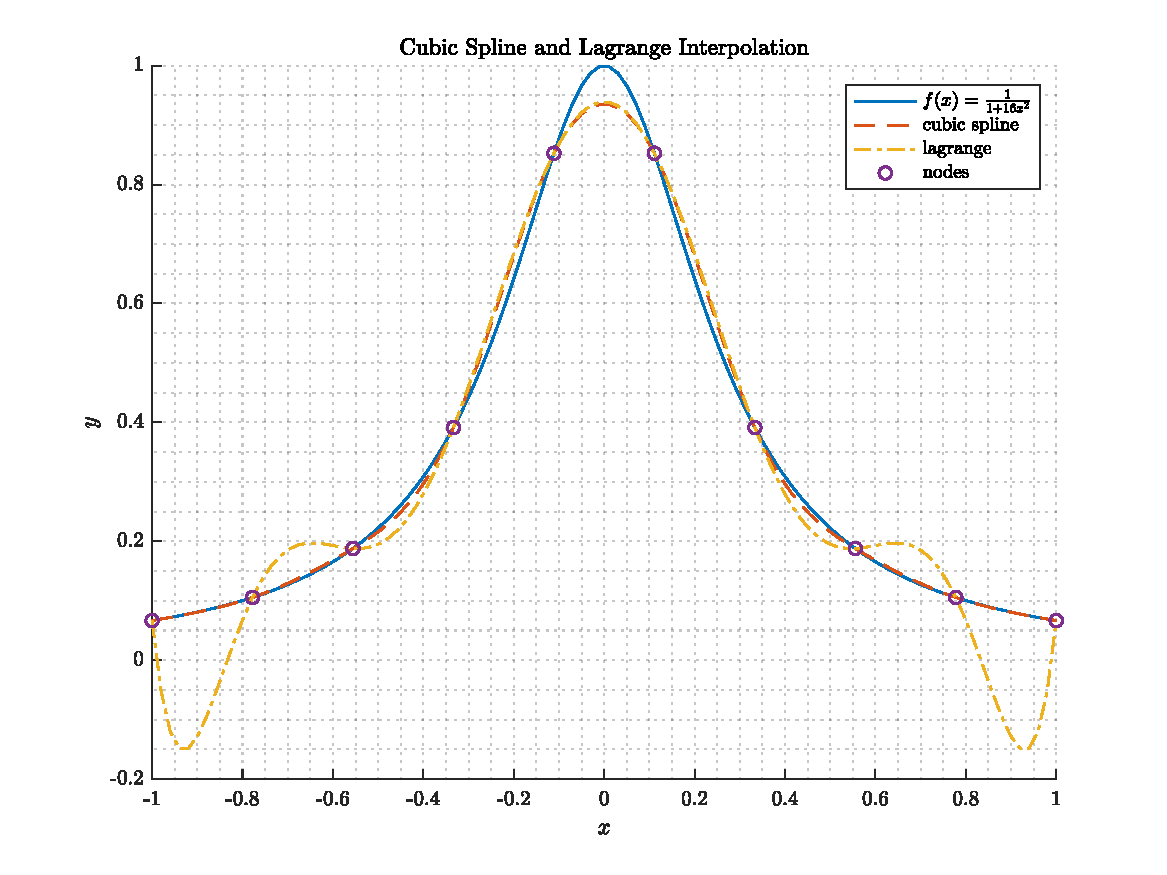
\includegraphics[width=0.75\linewidth]{../src/hw6_p2.pdf}
        \caption{Data Points, Cubic Spline Interpolant, and Polynomial Interpolant}%
        \label{fig:p2}
      \end{figure}
  \end{itemize}
\end{solution}

%%%%%%%%%%%%%%%%%%%%%%%%%%%%%%%%%%%%%%%%%%%%%%%%
% Problem 3
%%%%%%%%%%%%%%%%%%%%%%%%%%%%%%%%%%%%%%%%%%%%%%%%
\section{Problem 3}%
\label{sec:problem_3}
Consider the function
\begin{equation*}
  f(x) = \frac{e^{x}}{1 + x^{2}}.
\end{equation*}
Evaluate the error in its first derivative $f'(0)$, computed using the central first derivative formula, for a step ranging from $\Delta x = 0.1$ to $\Delta x = 10^{-7}$; decrease the value of the step $\Delta x$ by  a factor of 10 (one order of magnitude) for each successive evaluation. Plot the error versus the step $\Delta x$ using a logarithmic scale on both axes. Repeat the same calculations for the second derivative $f''(0)$, also computed with the centered formula. You may find that for some values of $\Delta x$ the error is zero; when using a logarithmic scale, this may lead to trouble when plotting, since the logarithm of zero is not defined (MATLAB does not complain, but Octave may produce an error message). To avoid this problem, you can just set the error to the machine accuracy \verb|eps| whenever it is lower than \verb|eps|.
\begin{solution}
  \quad
  \begin{itemize}
    \item
      Function file \verb|central_difference.m|
      \lstinputlisting[style=MATLAB]{../src/central_difference.m}
    \item
      Script file \verb|hw6_p3.m|
      \lstinputlisting[style=MATLAB]{../src/hw6_p3.m}
      \newpage
    \item
      Figure files: \verb|hw6_p3_1.pdf| (Figure \ref{fig:p31}) and \verb|hw6_p3_2.pdf| (Figure \ref{fig:p32}).
      \begin{figure}[!hbtp]
        \centering
        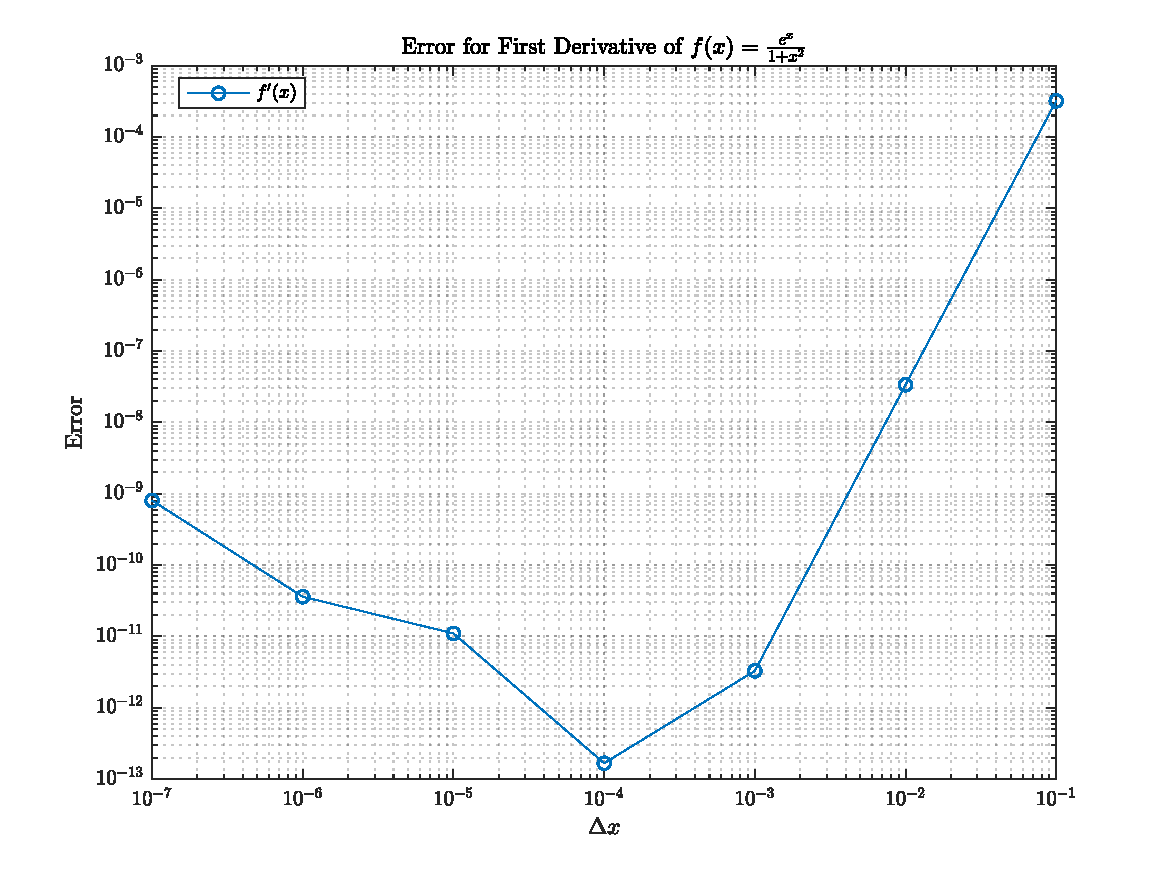
\includegraphics[width=0.75\linewidth]{../src/hw6_p3_1.pdf}
        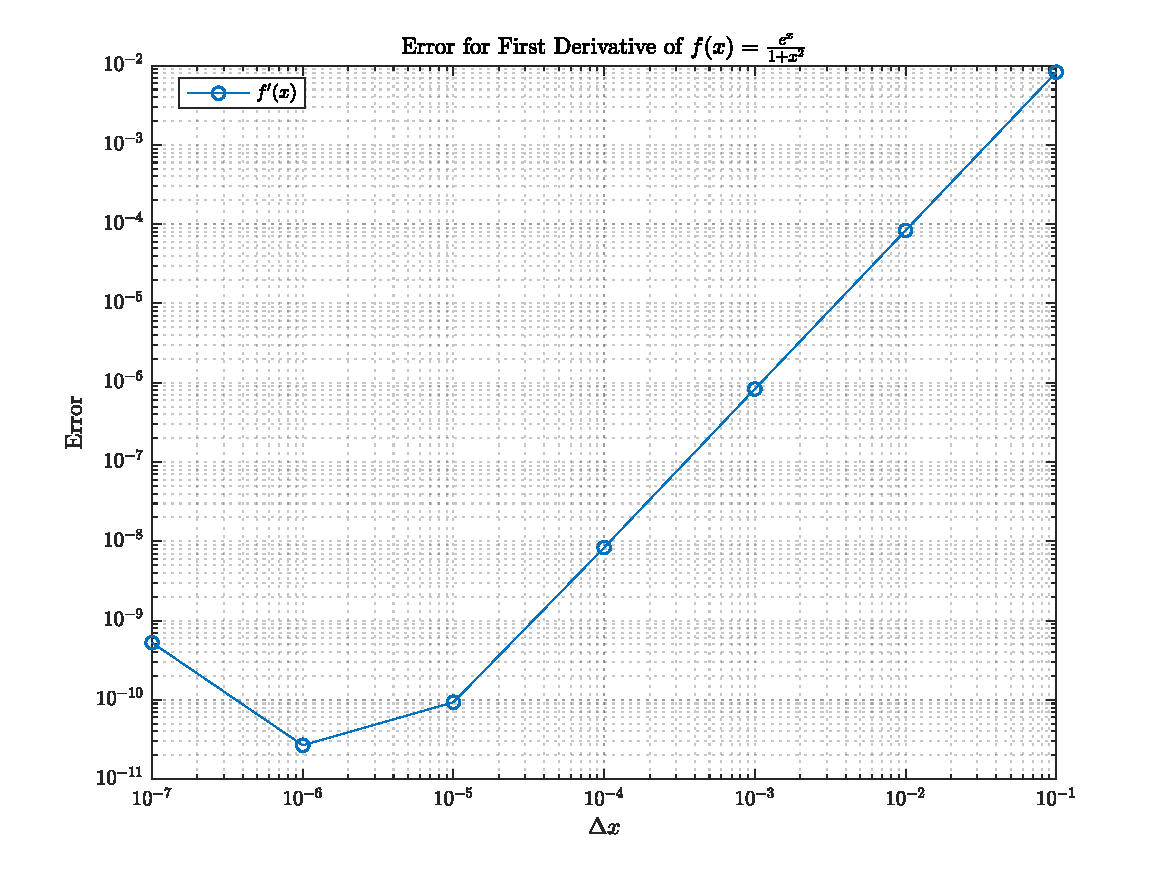
\includegraphics[width=0.75\linewidth]{../src/hw6_p3_3.pdf}
        \caption{Error vs. Step $\Delta x$ for First Derivative $f'(0)$}%
        \label{fig:p31}
      \end{figure}
      \begin{figure}[!hbtp]
        \centering
        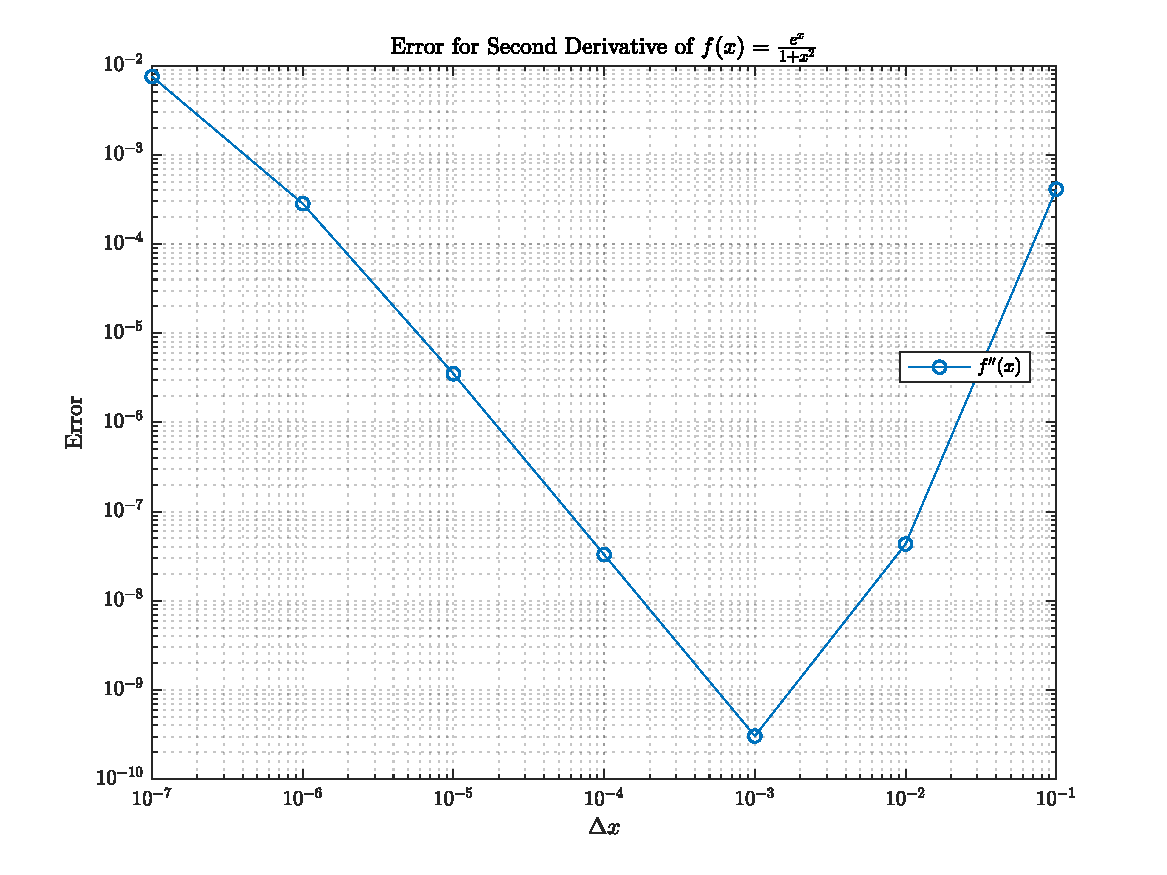
\includegraphics[width=0.75\linewidth]{../src/hw6_p3_2.pdf}
        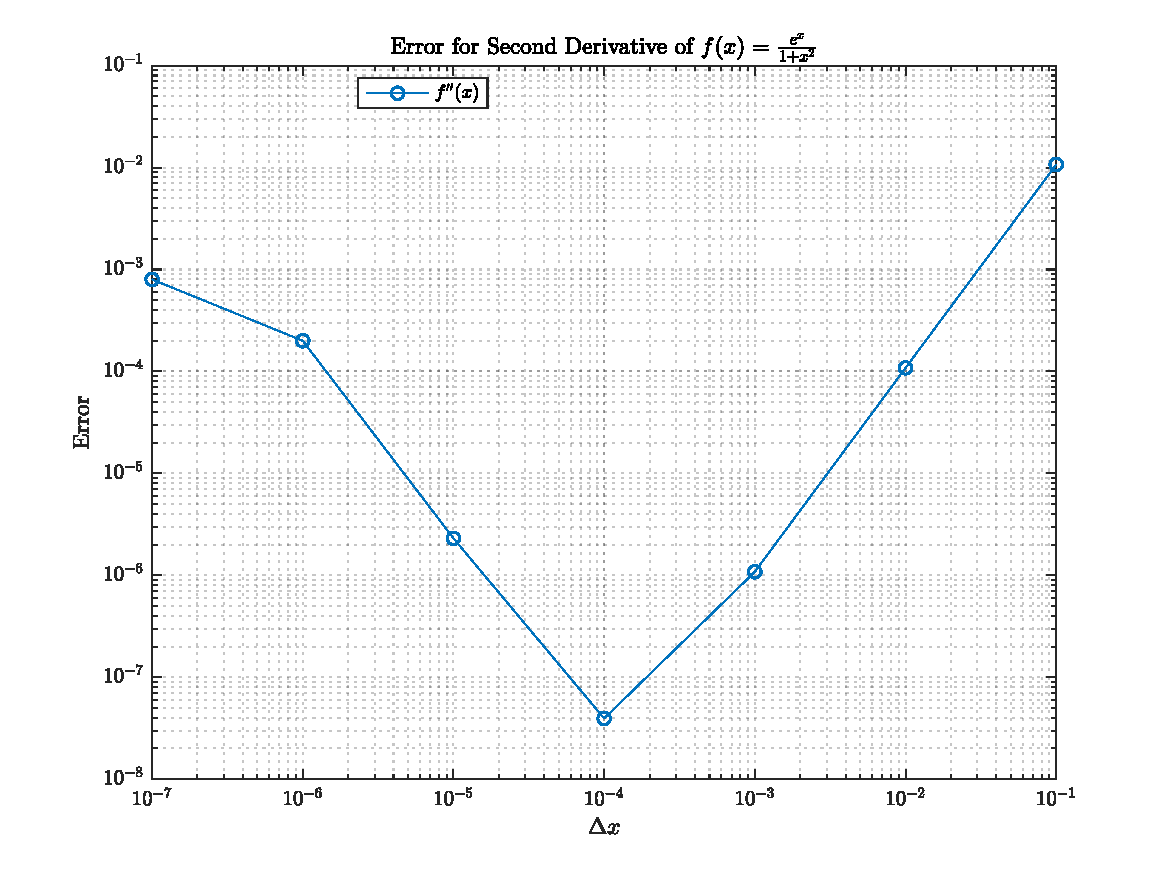
\includegraphics[width=0.75\linewidth]{../src/hw6_p3_4.pdf}
        \caption{Error vs. Step $\Delta x$ for Second Derivative $f''(0)$}%
        \label{fig:p32}
      \end{figure}
  \end{itemize}
\end{solution}

%%%%%%%%%%%%%%%%%%%%%%%%%%%%%%%%%%%%%%%%%%%%%%%%
% Problem 4
%%%%%%%%%%%%%%%%%%%%%%%%%%%%%%%%%%%%%%%%%%%%%%%%
\section{Problem 4}%
\label{sec:problem_4}
Using the Taylor series method set up in class (see section 7.2, page 117 in the typed notes) find a formula that approximates the values for $f'(x)$ and $f''(x)$ with the highest accuracy possible using a linear combination (weighted sum) of the values:
\begin{equation*}
  f(x - 2h), \quad f(x - h), \quad f(x + 2h), \quad f(x + 3h),
\end{equation*}
where $h = \Delta x$ is the step size. Do this calculation by hand.
\begin{solution}
  Results:
  \lstinputlisting[style=Plain]{../src/hw6_p4.txt}
  \lstinputlisting[style=MATLAB]{../src/hw6_p4.m}
\end{solution}
